\part{Histoire}

\chapter{Chronologie humaine}

\begin{multicols}{2}

\begin{center}
	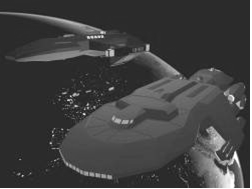
\includegraphics[width=150pt]{image/vaisseau5.png}
\end{center}

\textbf{De nos jours  – 2115 :} Montée en puissance des multinationales. Fondation des grandes nations :  
- l’alliance Américaine qui regroupe l’Amérique du nord et l’Amérique du sud.
- la fédération européenne contenant l’Europe et les pays au bord de la méditerranée. 
- l’empire d’orient, qui contient la chine ainsi que le Japon.
- l’union Africaine, qui existe officiellement sans vraiment fonctionner, cette union n’a aucun pouvoir…

\textbf{2083 – 2121 :} Nouvelle course aux étoiles. Fondation de multiples colonies spatiales.

\textbf{2094 :} L’alliance Américaine lance le programme « Nouveaux Mondes ». D’immenses vaisseaux-mondes capables d’atteindre la moitié de la vitesse lumière sont envoyés vers des étoiles lointaines notamment vers Proxima et Alpha du Centaure.

\textbf{7 Décembre 2125 :} Début du plan de terraformation de Vénus.

\textbf{5 Mars 2161 :} Premier contact avec des extraterrestres : les Ergios. Ils proposent à l’Europe de rentrer dans la fédération galactique au nom de la terre. Développement de la technologie Portail sur un chantier, près de la base spatiale européenne.
 
\textbf{13 Juin 2163 :} L’Afrique demande des comptes à l’Europe au sujet des Ergios. Le gouvernement nie avoir connaissance d’une race extraterrestre. 
 
\textbf{15 Juin 2163 :} L’alliance américaine apprend l’existence du chantier près de la base spatiale. 

\textbf{1 Juillet 2163 :} Prise de contrôle du chantier « Portail » par une attaque combinée de l’alliance Américaine, de l’empire d’orient, et de l’Union Africaine. 

\textbf{23 Janvier 2165 :} Fin de la construction du portail par le regroupement des grandes nations. Envoi d’un vaisseau ambassade.
 
\textbf{28 Janvier 2165 :} Retour de l’ambassade. La fédération est composée des Ergios, des Teldrims, des Snagirs, et des Vélïos. Les ambassadeurs ont également retrouvé les humains du programme « Nouveaux Mondes » qui ont été recueillis par les Ergios.

\textbf{2166-2219 :} Appartenance à la fédération qui ne semble pas si prometteuse que ça : les Ergios contrôlent tout ce qu’il s’y passe. 

\textbf{2218 :} L’empire d’orient s’allie avec les Vélïos.
 
\textbf{Fin 2219 :} Développement des nouvelles armes (dont les Méchas) en Europe avec l’aide des Ergios. Très vite chaque grande nation développe sa propre gamme basée sur la même technologie !
 
\textbf{2220 :} Début de la guerre intergalactique opposant les Vélïos, les Teldrims, les Terriens (Europe exclus) contre les Ergios et la fédération.

\textbf{2222 :} Repli des Vélïos sur leur propre territoire. Attaque des Américains contre les Européens. 

\textbf{2223 :} Exil inexpliqué des Ergios.
 
\textbf{Fin 2305 :} Restructuration de la fédération à l’initiative des Snagirs et de l’Europe. 

\textbf{2362 :} Fondation de la FFAC

\textbf{Juin 2369 :} Attaque de Kaitos par une flotte d’origine inconnu. Réouverture des communications avec l’Empire Vélïos.

\textbf{Juillet 2369 :} Conquête d'Ash'Nemba par l'alliance Kaitienne.

\textbf{Octobre 2369 :} Bataille de Phecda. Destruction de la fédération.

\end{multicols}

\chapter{Histoire Humaine}

\begin{multicols}{2}

\section{Une Ère d’Alliance}

Au début du XXIème siècle, la terre semble séparée en deux mondes totalement différents. D’un coté, les pays pauvres ou en voie de développement connaissent famine, maladie et guerre. Les nations pauvres sont sans cesse déchirées par des guerres civiles toujours plus longues les une que les autres.

A coté de ce monde où tout semble perdu, les pays riches connaissent une ère de bouleversement sans précédent appelée couramment la mondialisation. Les grandes puissances de la planète sont en paix depuis la seconde guerre mondiale et cette situation ne semble pas prête de changer. La mondialisation incite les pays à ouvrir leurs frontières et à diminuer le contrôle qu’ils exercent sur leur propre économie.

Les entreprises internationales, grandes gagnantes de cette époque, en profitent pour assoir leur influence au niveau mondial. Le pouvoir économique de ces entreprises devient si important que les gouvernements perdent tout pouvoir d’opposition et deviennent totalement indépendants. Peu à peu le monde développé se plonge dans une crise sociale, la faille entre les riches et les pauvres devenant chaque jour plus importante.

Pour contrer cette perte d’influence, les nations se regroupent, formant des organismes politiques importants capables de contrebalancer le pouvoir économique des multinationales et de faire pression pour rétablir la situation. 

Le premier bloc à former une alliance fut l’Union Européenne. Après plusieurs essais infructueux, les pays européens fondent le 17 février 2031 la Fédération Européenne, un tout nouveau gouvernement fédéral donnant un pouvoir fort à l’assemblé européenne. A cette époque la fédération regroupe l’intégralité des pays européens ainsi que les pays entourant le bassin méditerranéen. En une petite année l’Europe redresse la barre et commence à sortir de la crise. 

Le 23 août 2042, les pays de l’Amérique du nord et les pays de l’Amérique du sud annoncent la fondation de l’Alliance Américaine. Officieusement cette alliance est déjà effective depuis plusieurs années. 

Devant ce succès, la Chine et l’Indonésie décident d’agir rapidement et envahissent, en moins de 10 jours, l’Inde, puis le Japon et annoncent la création de l’Empire d’Orient le 9 juin 2045. L’Empire tente ensuite d’attaquer l’Australie. Toutefois, les deux autres grandes puissances réagissent et apportent leur soutien à l’Australie qui repousse aisément les armées Orientales, stabilisant la situation. L’empire est maintenant par la force malgré les protestations des Européens et des Américains. Toutefois la Chine possède l’arme nucléaire et les forces en présences n’osent pas déclencher une nouvelle guerre.

Pour éviter de sombrer davantage dans la pauvreté, les pays africains se regroupent peu à peu et forme l’Union Africaine. Cette union est plus une union de principe qui a pour but de limiter la guerre qu’un véritable gouvernement commun.

\section{La Course aux Etoiles}

En parallèle de ces évènements, les gouvernements se relancent dans la course aux étoiles, canalisant l’énergie de la société et ces moyens technologiques dans un seul et unique but : être les premiers à coloniser l’espace. La multiplication des gouvernements internationaux amplifie encore les moyens mis en œuvre et permet la multiplication des essais.

Les gouvernements progressent dans l’espace en suivant plusieurs axes :
\begin{itemize}
	\item Création de stations spatiales d’abord en orbite de la terre, puis plus lointaines dans l’espace..
	\item Colonisation des planètes proches grâce à l’utilisation de dômes spatiales.
	\item Recherches concernant la terraformation de Vénus. 
\end{itemize}


En 2094 l’alliance Américaine fonde le programme « Nouveaux Mondes ». Ils envoient une dizaine de gigantesques vaisseaux prévus pour vivre de façon autonome pendant une vingtaine d’années vers Proxima et Alpha Centauri. Après une accélération durant un mois, ces vaisseaux sont capables d’atteindre la moitié de la vitesse lumière. Ils devraient donc arriver à Centauri en à peu près 10 ans.

L’évènement le plus important de la colonisation spatiale a lieu le 7 décembres 2125. Alors que les plans de terraformation menés par l’Europe et l’Amérique semblent au point mort, l’empire d’Orient, resté plutôt discret jusqu’à maintenant sur ce sujet, met en place son propre programme et débute la terraformation de Vénus avec succès ! Toutefois le processus prendra une trentaine d’années avant de montrer des résultats satisfaisants. Cet évènement révolutionnaire amène la population terrienne, principalement les riches, à acheter des parcelles de terrains sur d’autres planètes ! Bien sûr, Vénus est déclarée comme territoire de l’Empire d’Orient ce qui déplaît fortement aux autres nations.

Les plus grandes corporations profitent de cette occasion pour rentrer dans la conquête spatiale et étendre leur marché exploitable aux colonies. Très rapidement le système solaire fut peuplé d’un grande nombre de bases spatiales en orbite d’une des planètes ou de ses satellites, voir même voguant librement dans l’espace et utilisant de petits moteurs pour éviter de tomber dans l’attraction de l’une des planètes. De nombreuses colonies furent établies et le trafic spatial devint quelque chose de routinier.

\section{Premier Contact}

Toutefois la terre n’eut guère le temps de se reposer sur ses lauriers car le 5 mars 2161, un étrange vaisseau s’approcha de la base spatiale militaire européenne de Déméter. Cet étrange vaisseau était une petite structure métallique à la forme arrondie dont la coque semblait sans cesse parcourue d’ondes électromagnétiques. Le vaisseau s’approcha et commença une procédure d’amarrage. La station voulut donner l’alarme mais les communications avaient été brouillées, tous dans la station crurent alors à une invasion.

Une fois amarrés, des êtres humanoïdes entièrement énergétiques et dont la forme semblait pouvoir varier selon leur volonté débarquèrent du vaisseau. L’une des formes prononça des mots qui furent compris par les membres de la station : « Nous ne sommes pas vos ennemis ».  Officiellement, les mots furent prononcés en Anglais, langue officielle européenne, toutefois les légendes urbaines racontent que les Ergios, car c’est comme ça qu’ils ont dit s’appeler, ont parlé une langue unique mais que chacun l’a entendue dans sa langue natale.

Les Ergios informèrent alors la capitaine de la base qu’ils étaient des diplomates envoyés par la grande Fédération Galactique, nommée Deneb Kaitos, ayant actuellement la régence d’une petite dizaine de systèmes solaires. Leur but de leur venue est de proposer aux terriens de rejoindre la fédération en tant que nation membre. Une fois leur annonce faite, les Ergios coupèrent leur système de brouillage et le capitaine de la station pu rétablir la communication et annoncer la nouvelle au QG.

Erwan Brenfeld, président Européen à l’époque de ces évènements, décida de garder cette information secrète et partit lui-même représenter la terre devant les Ergios. L’information ne fut même pas divulguée aux autres nations terriennes. Erwan questionna les Ergios pendant plus de deux jours avant d’accepter leur offre. En échange les Ergios s’engageaient à aider la terre à développer leur système de propulsion galactique pour que la terre puisse avoir ses représentants au sénat de la fédération galactique. L’accord fut signé et les Ergios travaillèrent alors de concert avec les scientifiques humains pour développer la technologie des portails. 

Le portail consistait en une énorme structure capable de générer un champ de force permettant aux vaisseaux qui le traverse de « plier l’espace-temps » (Loi de la Relativité) et de se déplacer presque instantanément vers un autre point. Au vue de l’énergie nécessaire et de la taille du mécanisme, Erwan décida de se servir de Déméter comme base pour le portail. Avant de partir, Les Ergios indiquèrent les coordonnées de Kaitos.

La fédération aurait pu alors être un avantage très important de l’Europe sur les autres nations si le 13 juin 2163 un pays membre de la fédération Africaine n’avait pas annoncé publiquement que le président Européen avait pris contact avec une race extraterrestre sans prévenir les autres nations terriennes. Le président Erwan nia totalement cette accusation.

Le 1er juillet 2163, la base Déméter fut attaquée simultanément par les flottes Américaines, Africaines, ainsi que celles de l’Empire d’Orient. La flotte de défense de la base fut totalement détruite. Le chantier tomba aux mains des autres nations qui apprirent toute la vérité et demandèrent des comptes à l’Europe. Le président Erwan ainsi que les principaux généraux de l’armée furent mis en état d’arrestation.

Pour la première fois depuis leur fondation, les quatre grandes nations se réunirent pour discuter. Après une longue délibération, il fut décidé de finir le chantier et de rejoindre la fédération galactique.

Pendant ce temps là, l’empire d’Orient avait profité que tous les yeux étaient tournés vers l’espace pour envahir l’Australie.

\section{L’Age Fédéral}

Le 23 Janvier 2165, la dernière pièce du portail, un gigantesque cristal fourni par les Ergios, fut mise en place. Le portail s’activa aussitôt. Un vaisseau transportant 4 ambassadeurs fut envoyé en direction de Kaitos avec pour but premier d’en apprendre un maximum de choses et d’évaluer la situation. 

5 jours plus tard le vaisseau revint avec l’intégralité de ces passagers, les bras chargés de photos (malheureusement totalement brouillées suite au passage dans les champs de force du portail), de souvenirs, … Les 4 ambassadeurs firent leur rapport dans un nouveau sommet mondial. Actuellement la fédération était composée de 3 races, sans compter les Ergios.

Les premiers d’entre eux sont les Snagirs. Les ambassadeurs les ont décrit comme des lézards de la taille d’un enfant humain. Ces lézards semblent particulièrement intelligents et sont considérés dans la fédération comme des puits de science. Toutefois, à première vue, leur peuple semble totalement désorganisé et orienté autour d’une structure clanique.

Les seconds sont les Teldrims, un peuple d’hommes chat. Chaque être de ce peuple peut être aussi différent d'un autre  que 2 chats terriens, tant au niveau de leur caractère, de la couleur de leur pelage voir de l’épaisseur de celui-ci. Pour l’instant, leur culture est un mystère. A première vue elle semble orientée autour d’un système de castez ainsi que d’une autorité religieuse forte. 

Et enfin les Vélïos, humanoïdez qualifiéz d’hommez-araignée par les ambassadeurs. Selon les rapports des ambassadeurs, la culture Vélïos est surement la plus proche de celle des humains. Ils semblent promptz à montrer leurs émotions qu’ils s’agissent de colère, de haine, ou d’amour. Leur société semble être organisée comme un empire, cela dit pour l’instant les ambassadeurs n’ont pas encore entendu parler d’un empereur Vélïos.

Ils annoncent que la communication au sénat est rendu possible à l’aide de traducteurs universels capables de traduire en instantané les paroles prononcées dans n’importe quel langage. Les ambassadeurs ont particulièrement été impressionnés par cette technologie et les Ergios ont accepté de leur donner les plans.

Et dernièrement, les ambassadeurs indiquèrent que la fédération galactique regroupe 11 systèmes solaires, en comptant la terre, dont 7 était devenu multiraciaux. Les Ergios ont d’ailleurs invité les humains à venir s’installer sur ces planètes.

C’est ainsi que la terre devint membre à part entière de la fédération galactique et qu’elle connut une nouvelle vague d’exil en direction des planètes de la fédération. Les multinationales (devenues alors corporations), comprenant très vite le filon représenté par ces nouvelles planètes, se jetèrent dans la conquête de ce nouveau marché. En l’espace de quelques mois, tout retour arrière sur la décision d’appartenance à la fédération était devenu impossible.

\section{La Guerre Galactique}

Une nouvelle vie s’établit autour de la fédération. Les humains reprirent très vite leurs vielles habitudes, cherchant toujours à obtenir un maximum de profits en dépit des autres membres de la société. Les corporations Teldrims et Snagirs réagirent très violemment (commercialement) à l’invasion des corporations terriennes ce qui provoqua une guerre économique dynamisant la vie sur les systèmes fédéraux.

Au fur et à mesure de leurs manigances, les humains se rendirent compte que la fédération était loin d’être démocratique. Les seuls maîtres à bord étaient les Ergios. Étant donné que la terre était déjà trop impliquée dans la fédération pour penser à un retrait, les politiciens terriens essayèrent de nouer des alliances dans le but de renverser les Ergios. Les Vélïos qui partageaient alors les mêmes idées sur la fédération devinrent des alliés de choix. Sur Terre, l’Europe s’opposa définitivement à ce projet.

En cachette, les Ergios contactèrent alors la fédération Européenne et leur proposèrent une aide technique dans le développement d’une toute nouvelle arme : les Mechas. Les Mechas sont des robots humanoïdes utilisant un système de contrôle à synchronisation synaptique partielle et permettant une très bonne précision dans le contrôle de l’engin. Cette arme révolutionnaire présentait un potentiel stratégique fort à cause de sa faculté d’adaptation, et, surtout, de l’effet de surprise. Malheureusement pour l’Europe, le projet filtra et les grandes nations développèrent toutes leurs propres gammes de Mecha. 

En 2189, une annonce des Vélïos et des Terriens déclara la guerre contre les Ergios dans le but de libérer la fédération de ces oppresseurs. L’Europe communiqua quelques minutes plus tard sa neutralité dans ce conflit. La première guerre galactique commença alors. La force alliée étant alors préparée au combat, les premières victoires furent remportées assez aisément. Toutefois les forces Ergios se réorganisèrent en quelques jours et la tendance fut inversée.

En fin d’année 2220, alors que les Ergios dominent à nouveau les champs de bataille, les Teldrims entrent également en guerre et se révoltent contre l’oppression Ergios. Cette nouvelle force permit de rééquilibrer un peu les camps, très vite la guerre s’enlisa. 

En début d’année 2222, les Vélïos, premiers alliés des humains, déclarèrent qu’ils se retiraient définitivement de cette guerre ainsi que de la fédération. Leur territoire devint totalement fermé, toutes personnes étrangères pénétrant dans leur système devenaient Persona non gratta et étaient abattues à vue. Et en effet, ce principe fut appliqué à tous les vaisseaux humains envoyés pour en apprendre plus. 

Le retrait des Vélïos fut un coup dur pour les forces alliées. Craignant alors que l’Europe ne tente d’en profiter pour prendre le contrôle de la planète Terre, les Américains décidèrent de porter une attaque éclair visant les principaux centres militaires européens. Toutefois l’opération n’eut pas le succès escompté, l’Europe repoussa les forces d’attaque et déclara la guerre à l’Amérique.

Très vite les Ergios reprirent le dessus. Tout semblait perdu quand, le 18 décembre 2223, les Ergios se replièrent et quittèrent totalement les territoires de la fédération. Aujourd’hui encore nul ne sait quelle est la raison de leur soudain retrait et tous craignent qu’ils ne reviennent lourdement armés.

\section{La Reconstruction}

Leur principal ennemi disparu, l’alliance vola en éclat et la Deneb entra dans une période d’anarchie, de guerre ouverte… Les grandes nations et les grands peuples s’affrontèrent essayant de s’accaparer les restes de ce qui avait été mis en place par les Ergios. L’anarchie dura plus de 80 ans… 80 ans au bout desquels l’action des diplomates Snagirs et Européens, combinée aux pressions mises en place par diverses corporations, arrivèrent à calmer la situation et à amener la création d’une nouvelle fédération : La Deneb Kaitos renaissait de ses cendres. 
Les textes de loi de la fédération furent rediscutés un à un, toute mention aux Ergios fut automatiquement supprimée. La fédération existe toujours mais est clairement amoindrie. Les Vélïos refusent toujours le moindre contact avec l’extérieur. Très vite le taux de criminalité augmente en flèche, les vaisseaux de guerre, rendus inutiles par ce semblant de paix, se reconvertissent à la piraterie.

Les Corporations font tout leur possible pour maintenir la situation. Vu le problème de criminalité, ils obtiennent le droit de posséder leur propre force militaire, droit que les plus grandes corporations vont utiliser pour bâtir des flottes à la hauteur de n’importe quelle flotte armée officielle. Les troubles ne se limitent pas à la fédération, l’autorité religieuse Teldrim est de plus en plus contestée au sein même de leur société. 

Dans la fin de l’année 2336, le laboratoire scientifique « Aurora Research » mené par le Snagir Sheeeliim déclare avoir réussi, pour la première fois dans l’histoire de la fédération, à déchiffrer des archives d’origine Ergios. Ces archives auraient révélé aux groupes de chercheurs les coordonnées du monde natal des Ergios : Ankaa. Ce monde aurait été abandonné il y a très longtemps par les Ergios, mais posséderait un portail de retour. 

Lors de la diffusion de leur résultat, le laboratoire n’a prit aucune précaution. Toutes les grandes puissances qu’elles soient nations, groupuscule pirate, ou corporations sont donc maintenant au courant des coordonnées exactes de ces nouveaux mondes. Cet évènement crée une lutte d’influence entre les différents groupuscules désirant profiter de la richesse de ces nouveaux mondes. Cette lutte s’est depuis très vite dégradée en guerre ouverte pour leur conquête et a faillit provoquer un nouvel éclatement de la Deneb. Les Centauriens, voyant défiler les flottes des guerres par leur système, réagissent promptement en limitant le passage des vaisseaux à de petits tonnages, permettant de stabiliser la situation.

\section{Nouvelle crise galactique}

En 2370, malgré les tentatives de restructuration, la fédération n’en reste pas moins une alliance plus que fragile où chacun essaye de faire un maximum de bénéfices. Qu’ils soient nations, corporations, ou même groupuscules criminels, tous se côtoient au sein de la fédération dans un équilibre instable. Le système solaire Ash’Nemba conteste de plus en plus le pouvoir de la fédération et de son président, peu à peu la population commence à parler d’indépendance. En réponse à ces rumeurs, la FFAC a déplacé ses forces dans le système d’Ash’Nemba pour, officiellement, combattre la forte présence pirate de ce secteur.

Alors que la force de la FFAC était mobilisée sur Ash’Nemba, une flotte Vélios très endommagée apparaît dans le système Kaitös. Une immense flotte d'origine inconnue la poursuit. Ce nouvel ennemi commence à bombarder et envahir la capitale.  Seule l'intervention de troupes armées de la SML permit de mettre à l’abri les représentants des différents systèmes. Finalement, l'alliance des forces Vélïos et Fédérales ont permit de repousser l'ennemi.

La flotte inconnue a toutefois réussi à fuir, effectuant un saut sans même rejoindre un portail ! Depuis il semble que les contacts diplomatiques entre la Fédération et les Vélïos aient repris, toutefois leurs frontières restent fermées. 

Les survivants témoignent avoir vu des êtres humanoïdes de taille humanoïde pourvus d’une immense paire d’ailes leur permettant de planer, voir de voler. La peau de ces êtres mélange les couleurs grises et violettes. Selon les témoignages, les armes de ces êtres étaient des armes à énergie directement greffées à même leur corps… 

Suite à cette attaque, le dirigeant de la Deneb orchestra l’annexion d’Ash’Nemba à l’Alliance Kaitéenne. Pour cela il simula à l’aide de troupes spéciales l’attaque d’Ash’Nemba par une bande pirate organisée et utilisa la flotte de la FFAC pour « protéger » le système. Le stratégème ne leurra personne, le président est trainé devant les cours de justice et destitué. Toutefois, l'alliance Kaitéenne refuse de libéré Ash'Nemba. La guerre éclate.

Les conflits reprennent avec une violence sans précédent. Les Snagirs menacéz, le Consortium Technologique réalise un cout d'état et réunit les Snagirs derrière un nouveau gouvernement fort et réactif. 

Le marché économique interstellaire commence à s'écrouler. En réaction les corporations fondent le Bureau Corporatiste. Plusieurs systèmes se placent sous leur protection. Le Bureau Corporatiste déclare la guerre à l'alliance Kaitéenne, responsable selon eux de la guerre. Très vite l'alliance Kaitéenne perd la capitale à leur profit. Le Bureau Corporatiste annonce également la découverte d'une technologie permettant le saut sans portail. Il refuse de partager cette technologie avec les autres gouvernements tant que la guerre durera. Mais cet argument ne semble pas convaincre les différents gouvernements de cesser les hostilités.

\end{multicols}

\chapter{Histoire Snagir}

\begin{multicols}{2}

\section{Ère de la fondation}

Les études historiennes Snagir sur leurs origines sont plutôt réduites, toutefois les Snagirs ont toujours gardé trace de leur passé dans la tradition orale, reste à trier le vrai du faux.

La période de l’ère de la formation correspond à la préhistoire humaine. A cette époque, les Snagirs devenait peu à peu l’espèce dominante de leur planète, utilisant et construisant des outils toujours plus perfectionnés.

Les Snagirs vénéraient alors Orchal, le dieu créateur ayant permis aux Snagirs d’évoluer. Pour les Snagirs, leur dieu n’était pas à l’origine du monde, mais il avait donné aux Snagirs, alors de simples animaux, une partie de sa divinité, leur permettant de gagner l’intelligence. Il semblerait que leur religion reconnaisse également un certain nombre de dieux mineurs, mais la tradition orale n’en a pas réellement gardé de traces.

C’est à cette époque que la civilisation a commencé à sa mettre en place, avec, en son centre, les grands prêtres d’Orchal considérés alors comme les véritables chefs de leur communauté. Déjà à cette époque, leur société semblait organisée selon un modèle pyramidal.

\section{Ère de la barbarie}

Les historiens estiment que la civilisation religieuse Snagir a réussi à survivre plus de 2000 ans, maintenant les Snagirs dans la paix et la prospérité. Bien que cette dernière ne soit pas contestée par les historiens, les Snagirs considèrent qu'à cette époque, leur peuple n’était rien d’autre que l'esclave de leurs dieux. 

Durant l’ère de la Barbarie, un autre dieu nommé Thorane gagna peu à peu des fidèles. Ce dieu offrait aux Snagirs l’indépendance vis à vis d’Orchal et de son panthéon esclavagiste pour leur donner le droit d’évoluer librement et de rejoindre les dieux dans le monde spirituel.

L’ordre religieux Snagir ne pouvait laisser passer cette hérésie, et très vite, une guerre de religion éclata. Il faut comprendre qu’à cette époque, l’intégralité de la société Snagir était organisée autour de leur religion.  De plus, une partie du peuple commençait à se lasser de l’ancien régime et voulait acquérir cette indépendance.

Cette guerre dura plus de 5 siècles et faillit mener les Snagirs à une extinction totale… Vers la fin de la guerre, les dieux furent considérés comme maudits et le peuple les renia. Toutefois, les Snagirs étaient toujours leurs esclaves.

\section{Ère impériale}

Puis vint Sssnack, le premier empereur éternel. Voyant son peuple mourir, Sssnack rassembla les foules sous sa bannière et entra dans la guerre religieuse comme une nouvelle force en présence. Son message était clair : les anciens dieux veulent la mort des Snagirs, pour survivre il faut donc les chasser de leurs terres. Le peuple le suivit très rapidement, et la guerre fut gagnée. Les historiens Snagirs considèrent avec sérieux que Sssnack a chassé les dieux de la planète. 

Au terme de la guerre, Sssnack, alors vénéré par le peuple, fonda l’empire. Toute religion fut totalement proscrite. Ce moment correspond au début des archives écrites chez les Snagirs.

Pendant tout son règne, Sssnack s’attacha à sauver son peuple et à mener une politique favorisant les naissances. Le peuple Snagir avait un besoin urgent de sang neuf pour survivre : toute leur civilisation était à rebâtir.

L’empereur siégea pendant plus de 120 ans, mourrant à l’âge exceptionnel de 175 ans. C’est de son âge avancé que lui vint le surnom de l’Empereur Eternel. Au moment de sa mort, il laissa derrière lui un peuple ayant reprit espoir et une société en cours de stabilisation, mais il ne laissa également aucun héritier. 

La société Snagir explosa à nouveau, laissant cours à une féroce guerre de succession. Cette guerre, toutefois moins meurtrière que la précédente, déboucha sur un millénaire d’anarchie.

\section{La renaissance}

\parpic[r]{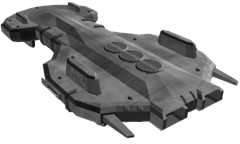
\includegraphics[width=100pt]{image/vaisseau6.png}} C’est dans cette longue période d’anarchie que commençèrent à se former les clans. Puis vint enfin une nouvelle réunification du peuple Snagir. Pour la première fois, les Snagirs expérimentaient un système où le peuple était son propre chef, un système démocratique qui est celui qu’on leur connaît actuellement. Ce système est basé sur un système de représentants pyramidaux élus par le peuple. Ce système, lent à réagir, a toutefois permit au Snagir de rester unis et en paix.

Durant cette période, les Snagirs se tournèrent vers la technologie. Leur niveau technologie connut un bond très impressionnant. 

Toutefois, cette évolution fut très vite ralentie par un principe de prudence : les premiers temps de cette évolution amenèrent leur lot de catastrophes technologiques majeures. Les Snagirs fondèrent de nombreux règlements pour éviter une évolution dangereuse. Aujourd’hui encore les chercheurs Snagir continuent à respecter ses textes ancestraux.

Depuis cette époque, la société Snagir resta relativement figée et calme.

\section{Ère fédérale}

Après une longue période de paix et de prospérité, les explorateurs Snagirs rencontrèrent des vaisseaux Ergios. Le premier contact fut très bref, mais également très pacifique. Les Snagirs avaient alors perdu toute velléité guerrière et cette rencontre les intriguait plus qu'elle ne les inquiétait. Un second contact fut établit plusieurs mois plus tard, et Snag'Isnar, président du Consortium Technologique, prit la parole au nom de son peuple. Après quelques semaines d'échanges et de négociations, un accord de paix fut conclut entre les deux puissances. A la découverte des Teldrims par les Ergios, les Snagirs soutinrent le projet de création d'une alliance tripartite solide, alliance qui fut les bases de la naissante fédération.

La plus grande particularité des Snagirs à cette époque est la facilité avec laquelle ce peuple a ouvert ses portes aux étrangers. Pénétrer et même habiter en territoire Snagir est assez aisé, même pour quelqu'un n'appartenant pas à leur race.

Puis vint la première guerre galactique, opposant les Humains, les Teldrims, et les Vélïos au peuple fondateur : les Ergios. Pendant toute la durée de la guerre, les Snagirs restèrent en dehors du conflit, se contentant de protéger leur territoire et leurs populations. Ils ne se prononcèrent jamais pour l'un des camps. Ce comportement fut conservé durant l'anarchie. Leur territoire grandit alors, mais uniquement suite à des demandes de protectorat de la part de leurs voisins...

Malgré leur absence de participation aux conflits, les peuples de la fédération ont apprit à ne pas sous-estimer la flotte Snagir qui possède une avancée technologique supérieure, et une discipline peu commune.

\end{multicols}

\chapter{Histoire Teldrim}

\begin{multicols}{2}

\section{Antiquité Religieuse}

L’antiquité Religieuse est le début de l’histoire connue des Teldrims. Il ne reste aucun savoir, aucun écrit, aucune trace de leur existence avant cet âge.

L’antiquité religieuse commence au moment où les dieux révélèrent leur existence aux 5 patriarches, leur révélant la raison de leur existence, la raison de leur diversité.

Chaque dieu prit un peuple sous son aile et avait pour rôle de les guider vers l’Anmara, le royaume mythique où les Teldrims retrouveront les dieux et vivront éternellement. 

Les dieux mirent également en garde leur peuple : à partir de ce jour les Teldrims devaient se transmettre de génération en génération l’histoire de leur peuple. Le jour où les Teldrims oublieraient leur passé, ils perdraient leur âme à jamais et ne pourraient plus rejoindre l’Anmara. Cet avertissement fut à l’origine de la caste des Prêtres, chargés de conserver, par tradition orale dans un premier temps, puis par écrit, leur us et coutumes ainsi que leurs légendes.

\section{L’âge de l’oubli}

Les différents peuples, chacun sous l’égide d’un dieu, vivaient en suivant son propre chemin. Les planètes avaient été séparées en 5 royaumes, un pour chaque espèce.

Peu à peu, le contact entre les peuples fut rompu, perdu, puis oublié. Les autres peuples étaient réduits à des êtres appartenant aux légendes… 

Oublié jusqu’au jour où chaque peuple avait tellement prospéré que leur territoire était devenu trop petit pour subvenir à leur besoin. Oublié jusqu’au jour où chaque peuple décida que son territoire n’était pas suffisant et qu’il était temps de l’agrandir.

C’est ainsi qu’une guerre meurtrière éclata entre les différentes espèces de Teldrim. Une guerre sans précédent. Une guerre qui dura des siècles et qui n’épargna personne.

\section{La mort d’un dieu}

Selon les légendes, c’est Ann’Nor, le dieu de la troisième lune, qui avait déclenché les hostilités en envoyant son peuple contre les plus faibles d’entre eux, les E’Rinims. 

La guerre devenait de plus en plus meurtrière et menaçait d’amener l’extinction des Teldrims dans leur ensemble. Les dieux se réunirent pour discuter d’une solution. Seul Ann’Nor fut rejeté par ses frères et ne put participer au conseil.

Durant cette réunion, les dieux decidèrent de frapper vite et fort. Ils envoyèrent toutes leur énergie contre leur frère reheté dans le but de le tuer et de libérer les Teldrims de son influence malfaisante. La troisième lune explosa, laisse une espèce Teldrim désamparée, sans guide.

Devant cet évènement, les 4 espèces encore guidées par un dieu s’allièrent et se retournèrent contre celle qui avait provoqué l’ire des dieux. 

Le peuple de la troisième lune fut vaincu. Les Teldrims auraient pu les exterminer mais ils décidèrent de leur laisser la vie. En échange, ce peuple qui avait perdu son guide avait perdu sa place : il devint un peuple esclave.

La fin des conflits arriva enfin. Les prêtres de tous les peuples se réunirent pour réorganiser les Teldrims et éviter qu’un tel conflit n’éclate à nouveau : ce fut la réunification.

Depuis ce jour, les prêtres ont toujours été l’élément liant les différentes espèces Teldrims en un seul et même peuple.

\section{Ère de la découverte}

La suite de l’histoire Teldrim est à la fois très riche de héros et de légendes, et très pauvre d’élémenta réellement bouleversants. 

La société Teldrim évolua doucement, la prêtrise s’arrangea pour conserver et implanter de façon durable les coutumes et les traditions. Le pouvoir de la prêtrise s’affermit jusqu'à devenir incontestable.

La prêtrise contrôlait le gouvernement, l'évolution, et l'histoire.

Les Teldrims s’élevèrent dans le ciel et colonisèrent les 4 lunes. Chaque lune était parfaitement vivable. Chaque lune devint le sanctuaire privilégie la prêtrise de l’espèce lié à elle. Puis les Teldrims s’étendirent doucement dans leur système solaire.

\section{L’ère fédérale}

Puis vinrent enfin les Ergios et leur message de paix. Les Teldrims virent l’offre des Ergios comme une porte vers l’Anmara. Ils acceptèrent sans condition et ne se rendirent compte que bien plus tard de leur erreur. Ils se rendirent compte que les Ergios n’étaient pas les messagers que leur dieux avaient choisis pour les emmener dans le royaume mythique.

Le début de la guerre contre les Ergios fut pour eux une libération et un nouvel espoir de trouver le chemin céleste.

\end{multicols}

\chapter{Historique Vélïos}

\begin{multicols*}{2}

\section{L’origine}

A l’origine, la planète mère des Vélïos a vu se développer deux races intelligentes, deux races dominantes. 

Les premiers-nés étaient les Eskadors, une race insectoïde possédant une faculté d’adaptation peu commune. Les second-nés étaient les Vélïos, une race à la force et à la résistance exceptionnels, une race dotée d’une paire de doubles lames.

Les deux races se sont développées ensemble, côte à côte, les Eskadors tempérant les ardeurs meurtrières des Vélïos et leur faisant profiter de leurs trouvailles technologiques, les Vélïos leur servant de main d’œuvre musclée pour les tâches où la force physique était nécessaire.

\section{Le schisme}

Nul ne se souvient pourquoi, mais un schisme apparut entre les deux races. Peu à peu, les Vélïos commencèrent à mettre à l’écart les Eskadors, à les isoler.

Le schisme s’intensifia, de plus en plus, avant de devenir une guerre, ou plutôt devraient-on dire, un massacre. Les Eskadors n’avaient aucune chance face au Vélïos, ils furent tués jusqu’au dernier. L’annihilation totale de leur espèce prit à peine un siècle.

Toutefois, il subsiste un doute… De nombreuses légendes Vélïos font référence à une lueur céleste qui serait venu intercéder en faveur des Eskadors et leur aurait permis de rejoindre un nouveau monde sous l’égide de leur dieu. Que cette légende soit réalité ou simple conte ayant pour but de donner bonne conscience aux Vélïos, la planète était totalement débarrassée de leurs confrères et les Vélïos étaient livrés à eux-mêmes.

\section{La régression}

Sans l’influence des Eskadors, les Vélïos se dispersèrent à travers leur monde en petites communautés survivant grâce à la chasse. Chaque communauté avait son propre territoire.

Le tempérament guerrier des Vélïos les incita bien vite à s’affronter régulièrement. Les Vélïos retombèrent totalement dans l’anarchie et dans le primitisme. 

\section{L’âge des Clans}

La régression dura des siècles avant qu’un semblant de civilisation ne luise à nouveau. Les tribus de chasse se regroupèrent peu à peu en groupes plus importants, formant des clans.

Les clans grossirent en nombre et en puissance, fusionnant parfois entre eux pour gagner de l’importance.

Peu à peu, une hiérarchie se fit entre les différents clans, la loi du plus fort commença à laisser place à une société plus structurée jusqu’à ce qu’il n’y ait plus qu’une dizaine de clans extrêmement puissants. Une dizaine de clans de force et d’influence équivalentes.

Mais la stabilité ne dura pas, les clans se lancèrent dans des combats acharnés et se disloquèrent à nouveau. Il devenait évident que sans une personne capable de dominer les clans, les Vélïos étaient voués à un combat permanent.

\section{L’Age Solaire}

L’âge Solaire commença par une catastrophe naturelle majeure, un évènement aujourd’hui encore inexpliqué parmis les scientifiques. Le soleil natal des Vélïos se mit à briller de milles feux, à envoyer beaucoup plus de rayonnements qu’ils n’en avaient connu jusqu’à maintenant.

Une grande partie des terres viables fut irradiées et devinrent d’immenses déserts. Les Vélïos périrent par milliers. Devant cette situation, les combats cessèrent et les Vélïos commençaient à s’entraider pour la survie de leur espèce. Les clans se reformèrent à nouveau.

Puis, un clan peu impacté par la catastrophe, le Shel’A’Vak, prit de plus d’importance. Ce clan était dirigé par une reine impitoyable, une reine à qui tous obéissaient sans discussion. Les humains l’auraient appellée tyran, mais les Vélïos l’appellèrent libératrice.

La reine profita de la puissance de son clan et de la situation délicate des autres pour imposer son pouvoir à tous et fonder un empire.

\section{L’Impératrice Éternelle}

\parpic[r]{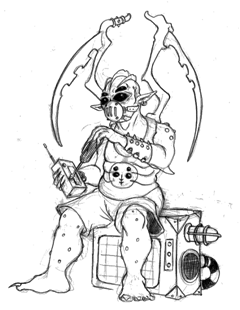
\includegraphics[width=100pt]{image/velios1.png}} Sous le règne de l’impératrice, les peuples Vélïos s’organisaient à nouveau et commençèrent à progresser y compris dans les domaines technologiques. Des moyens furent trouvés pour rendre à nouveau les zones sinistrées habitables.

Puis le peuple Vélïos se rendit dans les étoiles. Ils colonisèrent assez rapidement leur système solaire ainsi qu’un système voisin, très proche, accessible en à peine un an via l’espace normal.

Les siècles ont passé et l’impératrice a continué à guider son peuple vers la prospérité.  Selon les Vélïos, depuis presque un millénaire, il s’agit toujours de la même impératrice qui les guide. Elle serait immortelle… Bien sûr, pour les membres des autres peuples, cela n’est qu’une supercherie et les Vélïos doivent surement changer d’impératrice sans s’en rendre compte.

\section{Ère Fédérale}

Le reste est une histoire connue. Les Vélïos ont rejoint la premier Fédération et ont profité de nombreuses évolutions technologiques. Puis, ils se sont alliés aux humains avant de battre retraite et de fermer leurs frontières : tout s’est fait uniquement sur l’ordre de l’impératrice qui a plein pouvoir et que tous les Vélïos respectent.

L’impératrice ne justifiant pas ces choix, ni auprès de son peuple, ni auprès des autres nations, l’empire Vélïos reste un mystère imperméable… Comment une société aussi tyrannique peut-elle durer un millénaire ?

\end{multicols*}
